\documentclass[10pt]{standalone}
\usepackage{commands}

\begin{document}
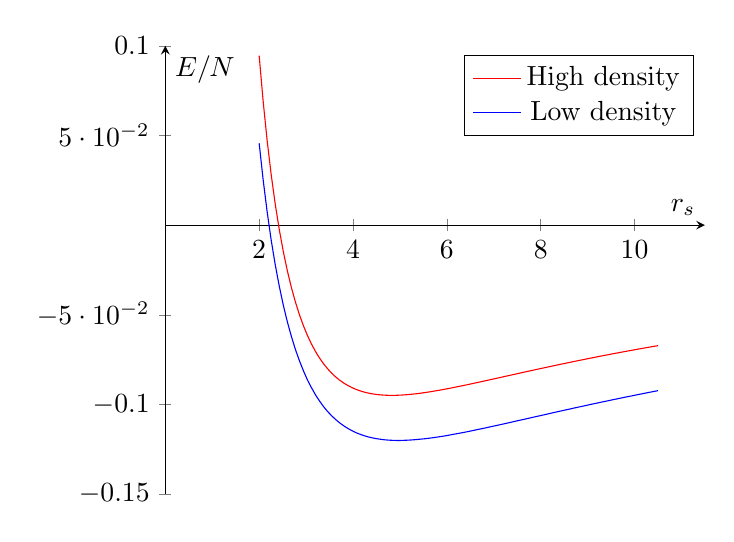
\begin{tikzpicture}
    \begin{axis}[axis lines=center,
        xlabel = \(r_s \),
        ylabel = \(E/N \),
        xmin = 0,
        xmax = 11.5,
        ymin = -0.15,
        ymax = 0.1]
    \addplot[domain=2:10.5,
    samples=100,
    color=red]{x^(-2) * (2.21 - 0.916*x)};
    \addlegendentry{High density}
    \addplot[domain=2:10.5, samples = 100, color = blue]{
        x^(-1) * (-1.79 + 2.66 * x^(-1/2))};
    \addlegendentry{Low density}
    \end{axis}
\end{tikzpicture}
\end{document}